\section{Motivating Examples}
\label{sec:motivating-examples}

We look at the namespaces of 3 applications.  Each is from different domains
and this list is not meant to be exhaustive. Similar organizations exist for
many domains, even something as distant as the mail application on a Mac. To
highlight the scalability challenges for file system metadata management, we
focus on large scale systems in high performance computing, high energy
physics, and large scale simulations. Large lists represent common problems in
each of these domains.

% This discussion is irrelevant since we are focusing on namespace size/overhead
%We benchmark over Ceph (Jewel version) with \(n\) object storage daemons
%(OSDs), 1 metadata server (MDS), 1 monitor server (MON), and 1 client.  We use
%3 OSDs because it sustains 16 concurrent writes of 4MB at 600MB/s for 2
%minutes. 250MB/s is the max speed of the SSDs, so the setup achieves 80\% of
%the cluster SSD bandwidth.  We use CephFS, the POSIX-compliant file system that
%uses Ceph's RADOS object store~\cite{weil:osdi2006-ceph}, as the underlying
%file system.  This analysis focuses on the file system metadata RPCs between
%the client and metadata server and does not include the RPCs needed to write
%and read actual data.  CephFS uses a cluster of metadata servers to service
%file system metadata requests~\cite{weil:sc2004-dyn-metadata} and to
%characterize the workload, we instrumented the metadata server to track the
%number of each request type\footnote{This code was merged into the Ceph
%project.}.

\subsection{High Performance Computing: PLFS}
\label{sec:plfs}

% What is the problem the authors are trying to solve?
Checkpointing performs small writes to a single shared file but because file
systems are optimized for large writes, performance is poor.  It easier for
applications to write checkpoints to a single file with unaligned writes of
varying length (N-1) but general-purpose distributed file systems are designed
for writes to different files (N-N).  The general problem is that the
application understands the workload but cannot communicate a solution to the
storage system. The common solution is for the file system to expose
configurations that describe alignment requirements but this forces application
developers to specify ``magic numbers" for parameters like write
size~\cite{bent_plfs_2009} or stripe size~\cite{behzad:sc2013-autotuning},
which are hard to find and may not even exist.  Another solution is to add
middleware ({\it i.e.} software that sits between the application and the
storage system) to translate the data into a format the storage system performs
well at. 

%% What is the problem?
%The problem is that the underyling file system cannot keep up with the metadata
%load imposed by PLFS. PLFS creates an index entry for every write, which
%results in large per-processes tables~\cite{grider:pc17-diddlings}. This makes
%reading or scanning a logical file slow because PLFS must construct a global
%index by reading each process's local index. This process incurs a
%\texttt{readdir} and, if the file is open by another process, an additional
%\texttt{stat()} because metadata cannot be cached in the
%container~\cite{bent_plfs_2009}.

%\subsubsection{System Architecture}
%@noah: there is an index because applications do not have regular IO

PLFS~\cite{bent_plfs_2009} solved the checkpoint-restart problem by mapping
logical files to physical files on the underlying file system. The solution
targets N-1 strided checkpoints, where many processes write small IOs to
offsets in the same logical file. The key insight of PLFS is that general
purpose file systems perform well for applications that use N-N checkpoints and
that the N-1 strided checkpoint style can be transformed with a thin
interposition layer. To map offsets in the logical file to physical files each
process maintains an index of \{logical offset, physical offset, length,
physical block id\}.  Each process sequentially writes to its own, unshared
data file in the hierarchical file system and records an offset and length in
an an index file. Reads aggregate per-process index files into a global index
file, which it uses as lookup table for logical file. 

% What is the authors' approach or solution?
%PLFS maps an application's preferred data layout into one that the file system
%performs well on. 
\subsubsection{Namespace Description}

% How does PLFS create namespaces
When PLFS maps a single logical file to many physical files, it
deterministically creates the namespace in the backend file system.  For
metadata writes, the number of directories is dependent on the number of
clients nodes and the number of files is a function of the number of client
processes.  A directory called a container is created per node and processes
write data and index files to the container assigned to their host.  So for a
write workload ({\it i.e.} a checkpoint) the underlying file system creates a
deep and wide directory hierarchy.

The namespace structure for 3 processes writing to variable offsets in a single
PLFS file is shown in Figure~\ref{fig:tree_plfs}. The \texttt{host*} directory
and \texttt{data*}/\texttt{index} files (denoted by the solid red line) are
created for every node in the system. The pattern is repeated twice (denoted by
the dashed blue line) in the Figure, representing 2 additional hosts.

\begin{figure}[tb]
\centering
  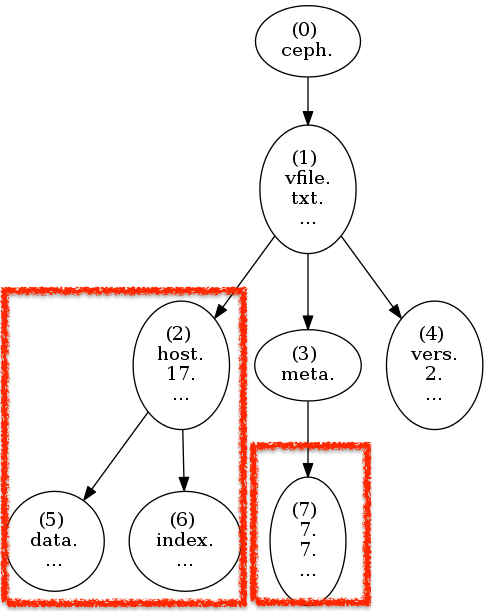
\includegraphics[width=1\linewidth]{figures/tree_plfs.png} 
  \caption{The PLFS file system namespace is structured and predictable; the
  pattern (solid line) is repeated for each hosts. In this case, there are three
  hosts so the pattern is repeated two more times. 
  }\label{fig:tree_plfs}
\end{figure}

\subsubsection{Namespace Size}

Figure~\ref{fig:plfs_problem} scales the number of clients and plots the total
number of files/directories (text annotations) and the number of metadata
operations needed to write out the PLFS file (``mkdir" and ``create") and to
read the PLFS file (``readdir" and ``open"). The number of files is \(2*n*m\)
for \(m\) servers and \(n\) processes per server. So for a 1 million processes
each checkpointing a portion of a 3D simulation, the size of the namespace will
be 2 million files just for the checkpoint. RPC-based approaches like IndexFS
have been shown to struggle with metadata loads of this size but decoupled
namespace approaches like DeltaFS report up to 19.69 million creates per
second, so writing checkpoints is largely a solved problem.

\begin{figure}[tb]
\centering
  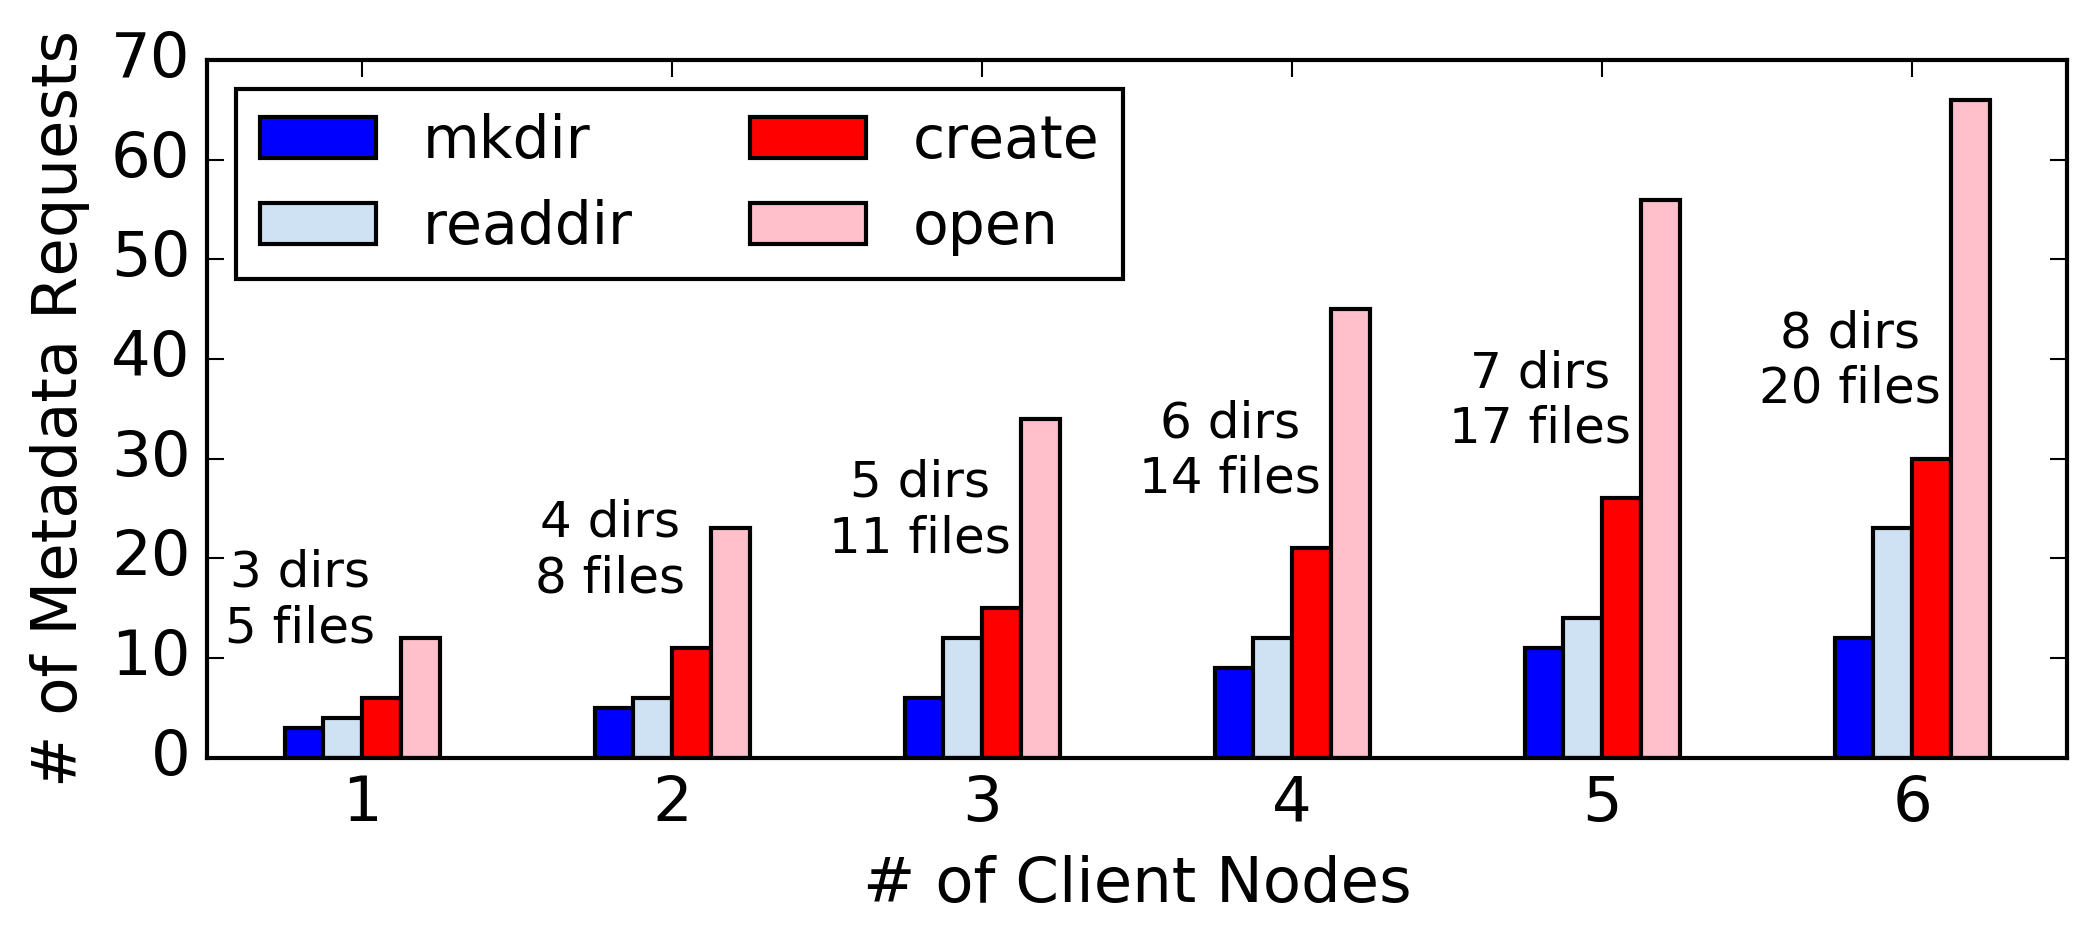
\includegraphics[width=1\linewidth]{figures/plfs_problem.png} 
  \caption{For PLFS, the file system  namespace scales linearly with the number
of clients.  This makes reading and writing difficult using RPCs so decoupled
namespace must be used to reduce the number of RPCs.  }\label{fig:plfs_problem}
\end{figure}

% How does PLFS read the namespace
For reading a checkpoint, clients must coalesce index files to reconstruct the
PLFS file. Figure~\ref{fig:tree_plfs} shows that the read metadata requests
(``readdir" and ``open") outnumber the create requests by about a factor of
\(4\times\) making RPCs even more untenable. Unfortunately, if the checkpoint
had been written with the decoupled namespace approach, file system metadata
would be scattered across servers (either clients or servers) so metadata would
need to be coalesced before restarting the checkpoint.  Current efforts improve
read scalability by reducing the space overhead of index
files~\cite{he:hpdc13-plfs-patterns} and transferring index files after each
write~\cite{grider:pc17-diddlings} but these approaches do not reduce the file
system metadata load and reading the index files still requires multiple RPCs.

\textbf{Takeaway}: the PLFS namespace scales with the number of client
processes so RPCs are not an option for reading or writing.  Decoupling the
namespace helps writes but then the read performance is limited by the speed of
transferring file system metadata across the network because metadata is
coalesced at the reading client.

\subsection{High Energy Physics: ROOT}

% the data
The High Energy Physics (HEP) community uses a framework called ROOT to
manipulate, manage, and visualize data about proton-proton collisions collected
at the large hadron collider (LHC). The data is used to re-simulate phenomena
of interest for analysis and there are different types of reconstructions each
with various granularities. The data is organized as nested, object oriented
event data and the length of the runs (and thus the number of events) are of
arbitrary length and type ({\it e.g.}, particle objects, records of low-level
detector hit properties, etc.).  Reconstruction takes detector conditions ({\it
e.g.}, alignment, position of the beam, etc.) as input.  Data is streamed from
the LHC into large immutable datasets, stored publicly in data centers around
the world.  Physicists analyze the dataset by downloading interesting events
stored in ROOT files.

\subsubsection{System Architecture}

% ROOT files
A ROOT file is a list of objects and data is accessed by consulting metadata in
the header and seeking to a location in the bytestream, as shown in
Figure~\ref{fig:tree_hep_a}. Scattered in the ROOT file is both data and ROOT
file specific metadata called Logical Record Headers (LRH).  For this
discussion, the following objects are of interest: a ``Tree" is a table of a
collection of events, listed sequentially and stored in a flat namespace; a
``Branch" is a data container representing columns of a Tree; and ``Baskets"
are byte ranges partitioned by events and indexed by LRHs.  Other objects, such
as ``Keys", ``Directories", and ``Leaves", contain HEP-specific metadata.
Clients request Branches and data is transferred as Baskets; so Branches are
the logical view of the data for users and Baskets are the compression,
parallelization, and tranfer unit. In summary, ROOT files are self-describing
files containing data located with metadata and serialized/de-serialized with
the ROOT framework.  Much of the development was done at CERN in parallel with
other HPC ventures. As a result, the strategies are similar to techniques used
in HDF5, Parquet, and Avro.

% WHat does ROOT have?
The advantages of the ROOT framework is the ability to (1) read only parts of
the data and (2) easily ingest remote data over the network.  Unfortunately,
the HEP community is running into scalability problems.  The current effort is
to integrate the ROOT framework with Ceph. But naive approaches such as storing
ROOT files as objects in an object store or files in a file system have read
amplification ({\it i.e.} read more than is necessary). Users would pull the
entire GB-sized blob to their laptop instead of reading metadata and Branches
a-la-cart. An alternative strategy that attempts to reduce read amplification
is the ``namespace approach"~\cite{pivarski:indico17-root}.

%\begin{itemize}
%
%  \item subdirectories within a file, for organization like HDF5
%
%  \item serialization of any type of C++ object, like Python's pickle, but for
%  C++
%
%  \item embedded schema with schema evolution like Avro
%
%  \item columnar storage of large sets of events, like the Dremel/Parquet
%  shredding algorithm (called "splitting" in ROOT)
%
%  \item selective reading, also like Dremel/Parquet (the "prune" feature of
%  SparkSQL DataFrames)
%
%  \item mutable content; a ROOT file is effectively a single-user object
%  database (but without ORM: the data are fundamentally not relational— maybe
%  "document store" would be a better word for what it's doing). Not all
%  operations are guaranteed to be atomic or thread-safe (hence "single-user").
%
%\end{itemize}
%
%Optimizations and trade-offs are controlled with configurations. For example,
%the \texttt{splitlevel} parameter controls the data layout, {\it i.e.} whether
%it is organized more closely to rowwise or columnar.  Low values store columns
%values as tuples in entries ({\it i.e.} \texttt{splitlevel=0} stores all column
%values as tuples in each entry) while high values make the data more
%columnar-based. Other parameters control the size and shape of hierarchical
%structure of the ROOT file include events per file, target Basket size, cluster
%size, compression algorithm and level, and alignment of objects with disk
%pages.

\subsubsection{Namespace Description}
\label{sec:hep_namespace-description}

\begin{figure}[t!]
    \centering
    \begin{subfigure}[b]{.45\linewidth}
      \centering
      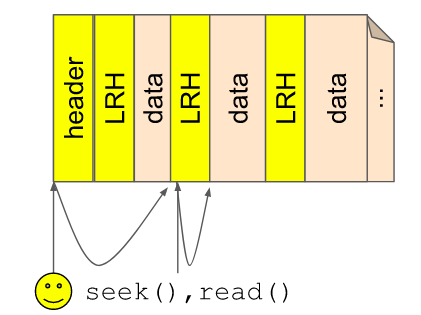
\includegraphics[width=1.0\linewidth]{figures/tree_hep_a.png} 
      \caption{file approach}
      \label{fig:tree_hep_a}
    \end{subfigure}
    \begin{subfigure}[b]{.45\linewidth}
      \centering
      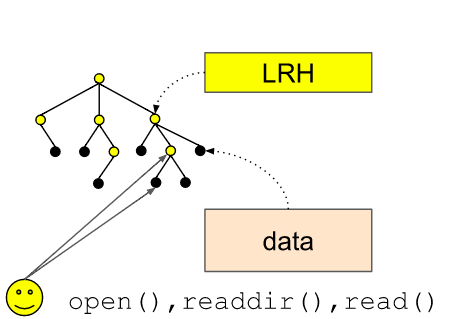
\includegraphics[width=1.0\linewidth]{figures/tree_hep_b.png} 
      \caption{namespace approach}
      \label{fig:tree_hep_b}
    \end{subfigure}
    \caption{(a) shows how the file approach for handling HEP data stores
everything in a single ROOT file, where the client reads the header and seeks
to metadata (LRH) and data. For ROOT files stored in distributed file systems reads will
have amplification because the system's striping strategies are not aligned to
Baskets. (b) shows how the namespace approach stores Baskets as files in the
file system namespace so clients read only the data they need.}
\end{figure}

The namespace approach views a ROOT file as a namespace of data. At the top of
the namespace are Keys, each containing pointers to groups of Branches. For
example, ``MetaData" has data about the run and ``Events" has all the
proton-proton activity. Physicists ask for Branches, where each Branch can be
made up of multiple subBranches ({\it i.e.} \texttt{Events/Branch0/Branch1}),
similar to pathname components in a file system file name.  To accomodate this
model, the namespace approach partitions the ROOT file onto a file system
namespace.  As shown in Figure~\ref{fig:tree_hep_b}, file system directories
hold Branch metadata and files contain Baskets. Clients only pull baskets
they care about, which prevents read amplification.  Unfortunately, storing
this metadata in a file system would overwhelm most file systems in two ways:
(1) too many inodes and (2) per-file overhead.  To quantify (1), consider the
Analysis Oject Dataset which has a petabyte of data sets made up of a million
ROOT files. If these ROOT files are split by Branches, there would be a billion
files. To quantify (2), we benchmark a simple ROOT workload over CephFS.

%is not enough metadata to reconstruct which Branches belong to which events.
%tely, current file system do not have this many inodes and this setup
%would require extra metadata to combine TBranches into objects.

\subsubsection{Namespace Size}

\begin{figure}[tb]
\centering
  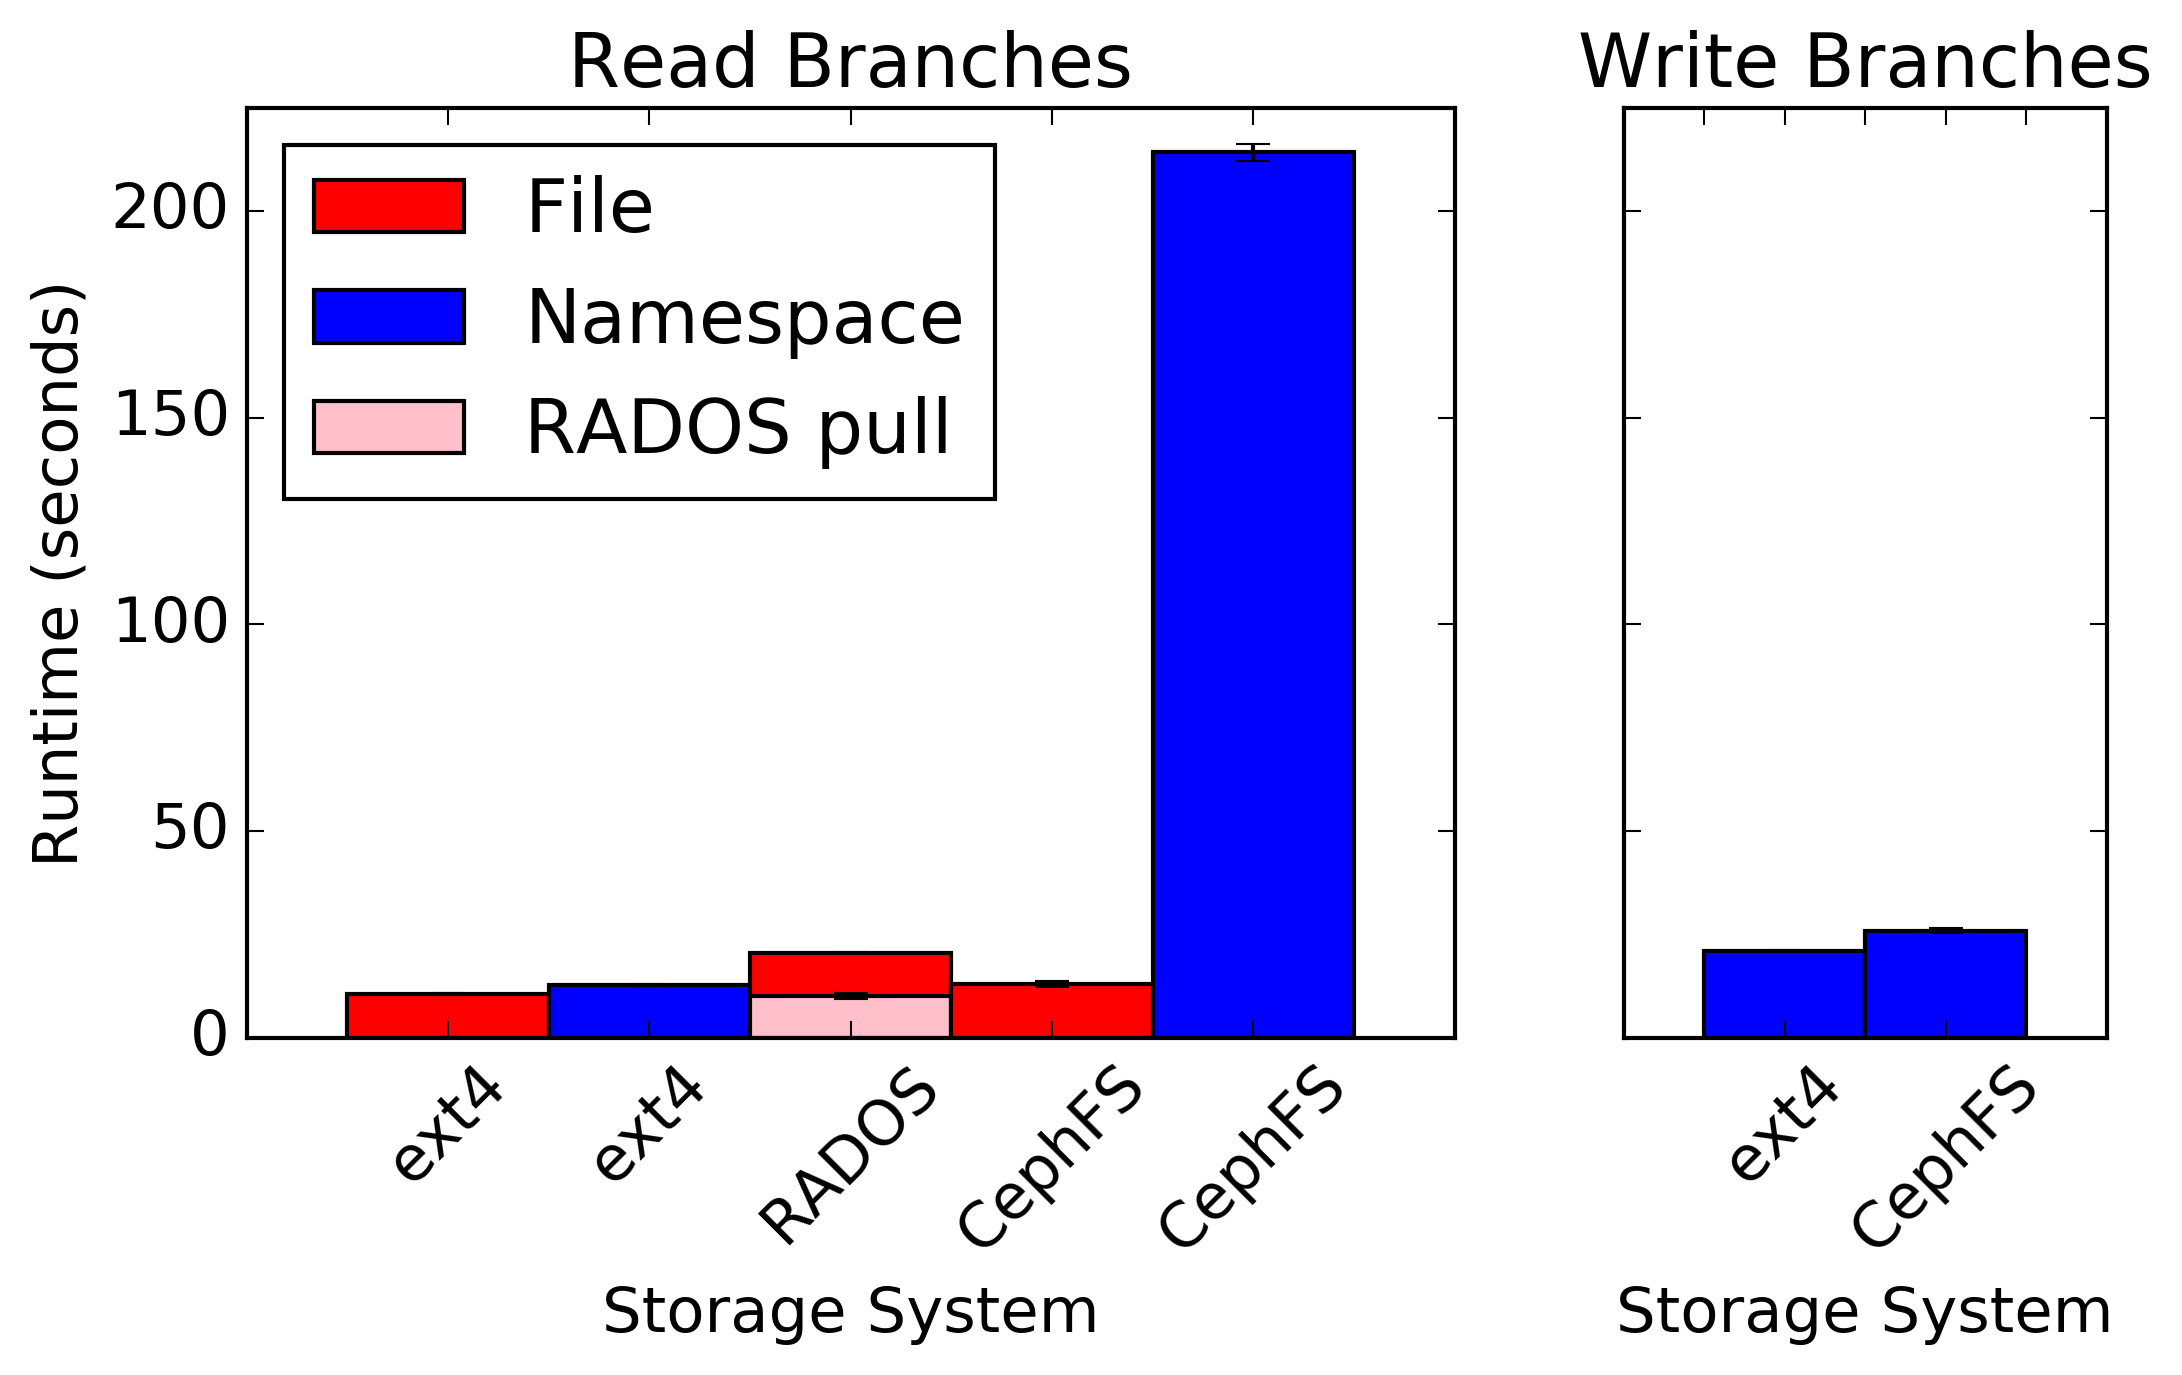
\includegraphics[width=1\linewidth]{figures/hep_runtime.png}
  \caption{ ``Namespace" shows the runtime of storing a file per Basket and
``File" shows the runtime of storing data as a single ROOT file. RPCs are
slower because of the metadata load and because many small objects are pulled.
Decoupling the namespace has less network (because only metadata and relevant
Baskets get transferred) but the benefit is offset by the cost of materializing
the namespace.} \label{fig:hep_runtime}
\end{figure}

%%\begin{figure}[t]
%%  \centering
%%  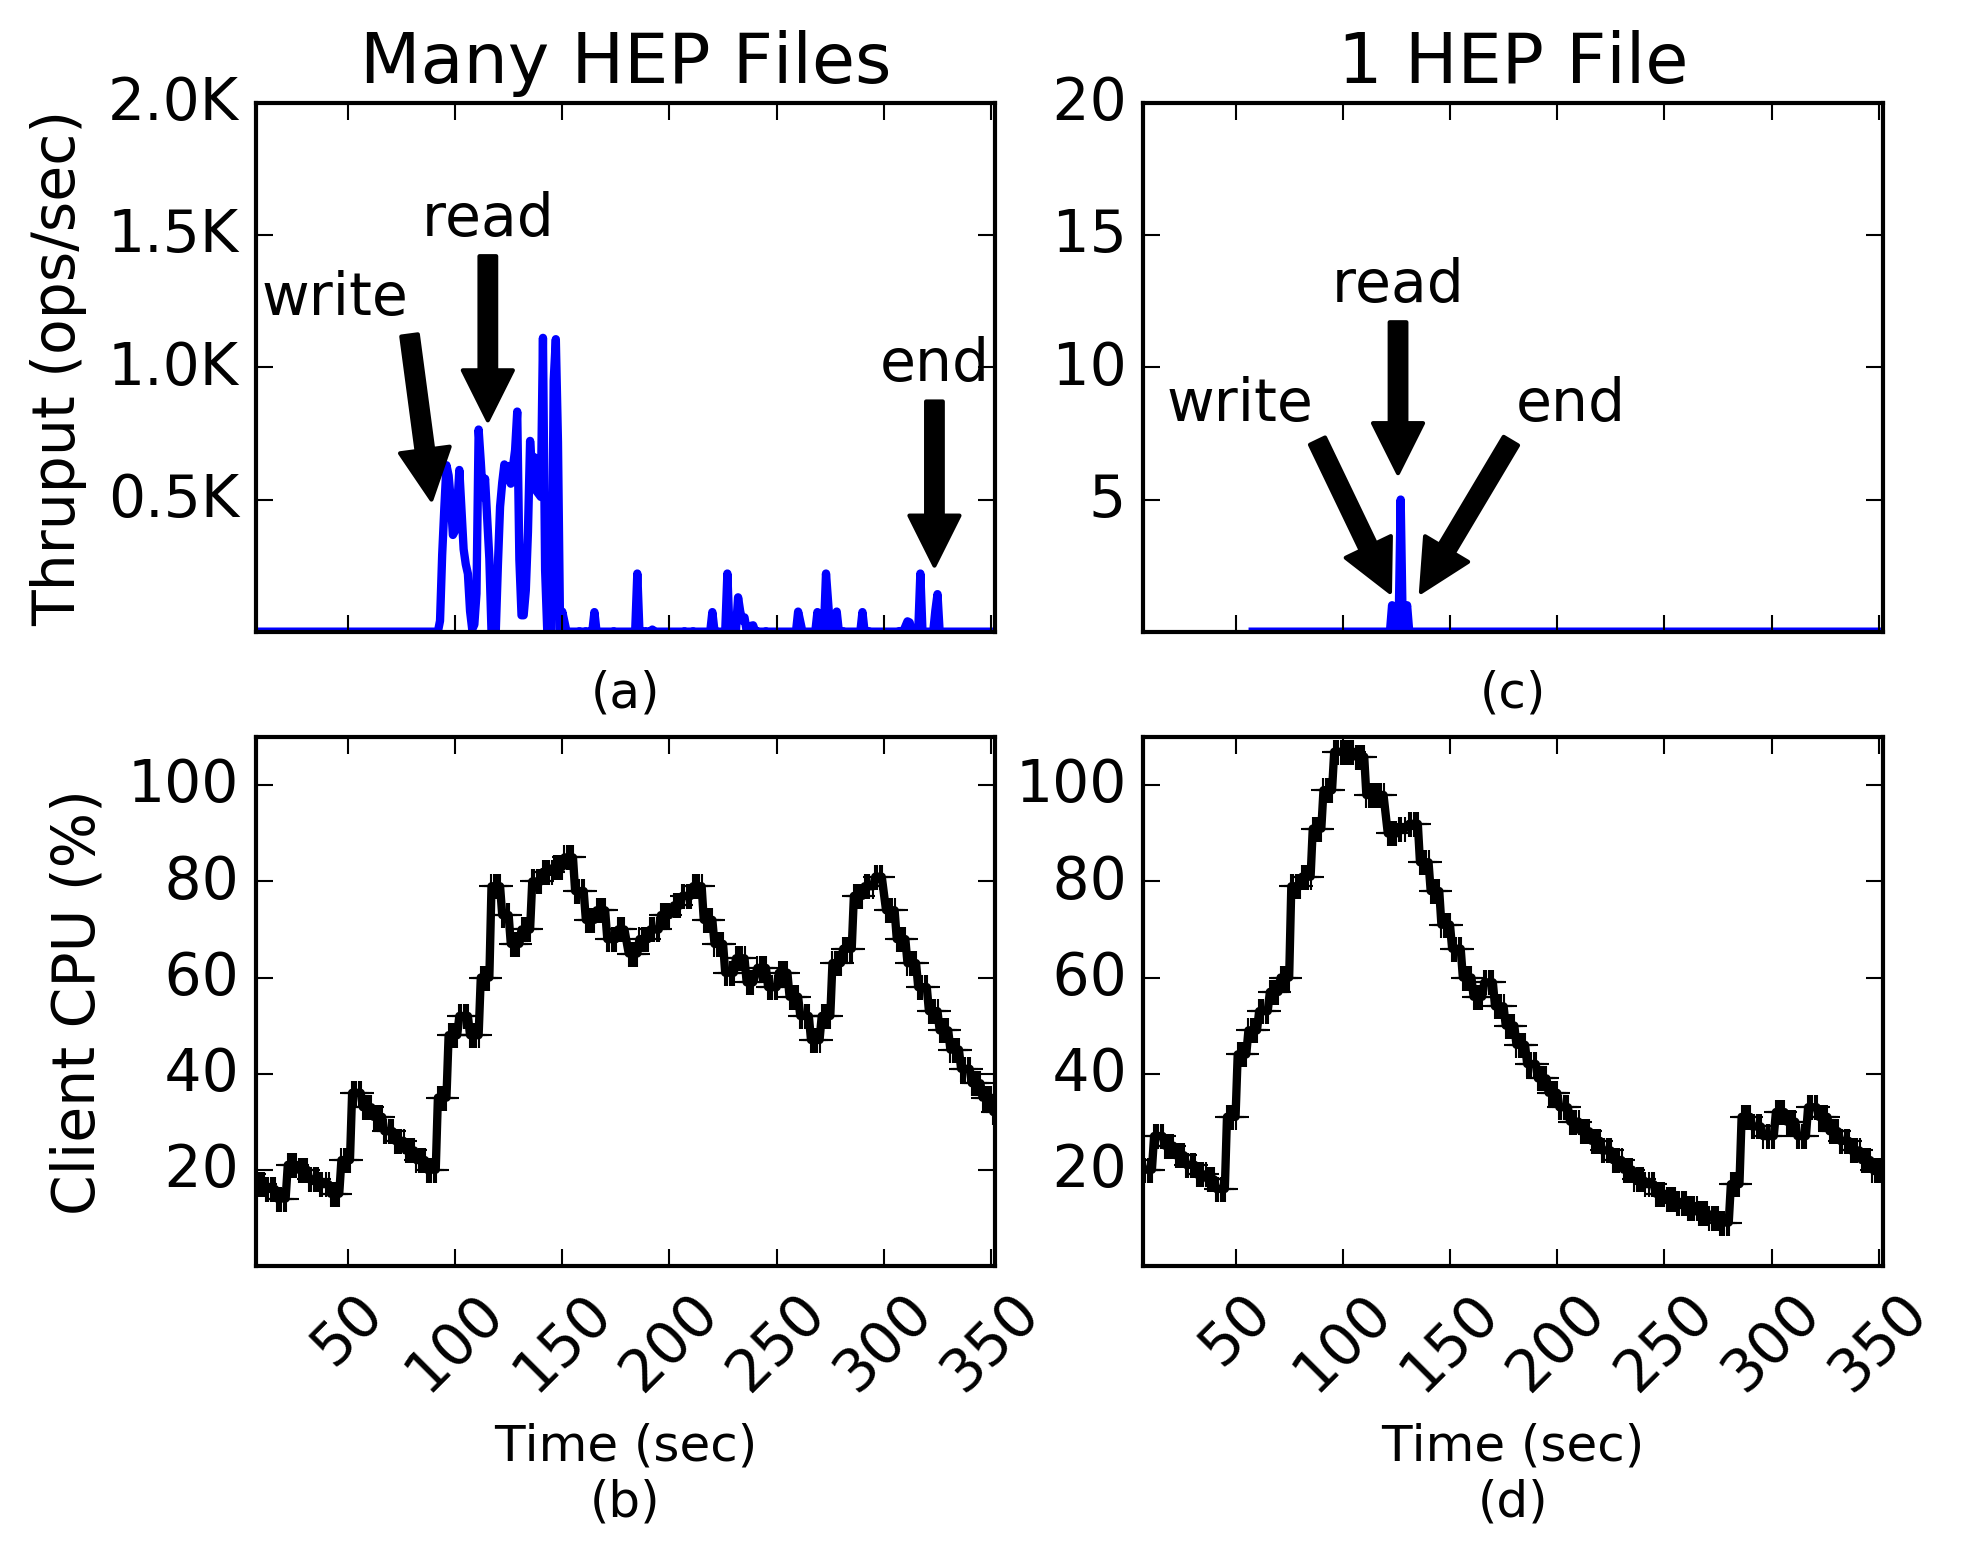
\includegraphics[width=90mm]{figures/hep_problem.png}
%%  \caption{Reading and writing high-energy physics (HEP) data as many files
%%allows physicists to read just the data they care about. But using this
%%namespace approach sends many RPCs to the metadata server (a), resulting in
%%worse performance and lower CPU utilization at the client (b). Alternatively,
%%using the traditional file approach has IO amplification because all data moves
%%over the network but less RPCs (c), better performance, and higher client CPU
%%utilization (d).}
%%  \label{fig:hep_problem}
%%\end{figure}

We benchmark the write and read overhead of storing HEP data with the file
approach stored as one object in an object store, with the file approach stored
as one file in a file system, and with the namespace approach stored as many
files in a file system.  The file approaches are deployed without any changes
to the ROOT framework. For the namespace approach, HEP-specific metadata is
mapped onto the file system namespace. In CephFS, Baskets are stored in Ceph
objects and the Branch hierarchy is managed by the metadata server.  Clients
contact the metadata server with a Branch request, receive back the Branch
hierarchy necessary to name the Ceph object containing the Basket as well as
the deserialization metadata necessary to read the object.  The workload is a
list of Branch accesses from a trace of the NPTupleMaker high energy physics
application. Each Branch access is:

\texttt{Branch0/Branch1,3,1740718587,5847,97,136}

where the tuple is the full Branch name, Basket number, offset into the ROOT
file, size of the Basket, start entry of the Basket, and end entry of the
Basket.  For the file approach, we use the offset into the ROOT file and the
size of the Basket.  In setup 1, the ROOT file is pulled locally and the
Branches are read from the file. In setup 2, the offset and size of the read
are sent to the CephFS metadata server.  For setup 3, the full Branch name and
Basket number are used to traverse the file system namespace.

%The start and end entry of the Basket are the logical records that
%bookend the Basket ({\it e.g.}, for a start entry of 10 and end entry of 20 for
%a Basket storing user ages, the start entry is user 10's age and the end entry
%is user 20's age).  

The read and write performance for the different approaches are shown in
Figure~\ref{fig:hep_runtime}, where the \(x\)-axis is approaches for storing
ROOT data, the \(y\)-axis is runtime, and the error bars are the standard
deviations for six runs. Using the namespace approach with RPCs is far slower
because of the metadata load and because many small objects are pulled over the
network. Although the file approach reads more data than is necessary since the
stripe size of the file is not aligned to Baskets, the runtime is still
\(16.6\times\) faster. Decoupling the namespace is much faster for the
namespace approach but the cost of materializing file system metadata makes it
slower than the file approach. 

%The reason is shown in Figure~\ref{fig:hep_problem}. The file system metadata
%accesses, characterized by many \texttt{open()} requests, incur many RPCs.
%This causes worse performance and lower client CPU utilization compared to
%reading a single ROOT file.  So the cost of read amplification in the file
%approach is offset by the cost of doing namespace operations. For this
%experiment, the ROOT file is 1.7GB and 65\% of the file is accessed so the
%namespace approach might be more scalable for different workloads.\\

\textbf{Takeaway}: the ROOT namespace stores billions of files and we show that
RPCs overwhelm a centralized metadata server. Decoupling the namespace helps
writes but then the read performance is limited by the speed of transferring
file system metadata across the network as clients read Baskets.  Read
performance is also limited by the cost of materializing and scanning parts of
the namespace that are not relevant to the workload.

\subsection{Large Scale Simulations: SIRIUS}

SIRIUS~\cite{klasky:journal16-sirius} is the Exascale storage system being
designed for the Storage System and I/O (SSIO)
initiative~\cite{ross:report14-ssio}. The core tenant of the SIRIUS project is
application hints that allow the storage to reconfigure itself for higher
performance. Techniques include tiering, management policies, data layout,
quality of service, and load balancing. 

\subsubsection{System Architecture}

SIRIUS includes a metadata service called Empress~\cite{lawson:pdsw17-empress},
which is a query-able SQLite instance that stores metadata for bounding boxes
({\it i.e.} a 3-dimensional coordinate space).  Figure~\ref{fig:empress} shows
how metadata is stored in and retrieved from Empress; the entire simulation
space, represented as a 3D torus, is partitioned into bounding boxes, whose
coordinates are stored in SQLite for each variable ({\it e.g.}, temperature,
pressure, etc.).  The objecter function, \(F(x)\), translates the bounding box
coordinates into a list of object names, which are used to write/read data
to/from the scalable object store. The use of the objecter avoids the need to
explicitly store object names; instead Empress only needs to store global
offsets for interesting features. SIRIUS aims to satisfy queries structured
like the ``Six Patterns in HPC"~\cite{lofstead:hpdc11-6degrees}. 

Empress is designed to be used at any granularity, which is especially
important for a simulation space represented as a 3D mesh. By granularity, we
mean that metadata access can be optimized per variable, per timestamp, per
run, or even per set of runs (which is possible but may require multiple
queries).  Empress is also designed to scale-out via additional independent
instances. In this distributed case, one client per server queries the entire
space of interest and shares results with other processes that may want the
same metadata. This process queries servers, coalesces results, and distributes
them using MPI messages.

%So clients reading from SIRIUS will first
%contact Empress with the queries for all data, all of 1 variable, all of a few
%variables, a plane in each dimension, an arbitrary rectangular subset, or an
%arbitrary area on an orthogonal plane, and Empress will return a list of
%objects. Armed with this list, the client contacts the object storage system
%(in our case this is RADOS, Ceph's object store) and reads relevant data.

\begin{figure}[tb]
\centering
  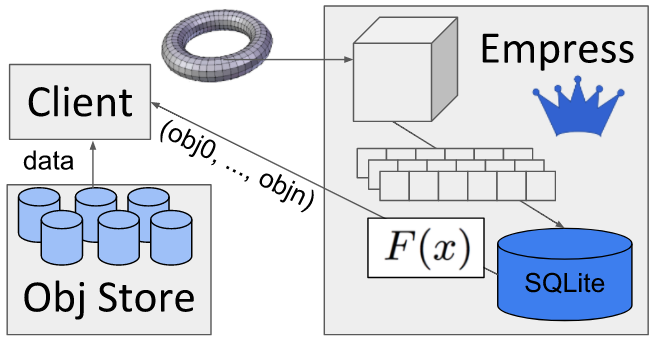
\includegraphics[width=1\linewidth]{figures/empress.png}
  \caption{The SIRIUS project uses Empress to store metadata for bounding boxes
in a 3D torus. Bounding box coordinates and a list of object names are stored
in SQLite. The object names are calculated using an objecter function, labeled
\(F(x)\) above. For reads, clients query Empress for the object list before
reading from the object store.}
  \label{fig:empress}
\end{figure}

\subsubsection{Namespace Description}

The seven columns in the database are six coordinates, which are integers
representing the contents at a location in the global space, and a string
representing the object name. The global space is partitioned into
non-overlapping, regular shaped cells.  Each row in the database is duplicated
for each variable in the simulation because variables may have a different
partitioning of the global space; for example temperature is computed for every
cell while pressure is computed for ever \(n\) cells.  Figure~\ref{fig:empress}
only has three variables, represented by the rows of boxes but most simulations
will have a minimum of 10 variables.

\subsubsection{Namespace Size}

To satisfy bounding box queries, Empress lists and filters relevant coordinates
before returning a list of (possibly overlapping) object names. The user
usually knows which bounding boxes are of interest by tagging features at write
time. So while the client does minimal filtering, aside from slicing objects at
the ``edge" of the bounding box, the internal Empress implementation is
bottlenecked by listing and filtering for coordinates \textcolor{red}{UGH is
this true? If so the objecter fxn doesn't solve this... I think the bottleneck
should be the cost of sending all those object names over the network!!!}
of interest. This is a problem because of the size of the object name list.
Listing large numbers of items in file systems is notoriously slow and studies
on \texttt{ls} have shown the operation to be especially
heavy-weight~\cite{carns:ipdps09-pvfs, eshel:fast10-panache}.  As currently
designed, Empress would store too many object names while the target query
types only request subsets of the resulting list.

\emph{\# of object names}: a back-of-the-envelope calculation for the number of
object names in the system is:
\[=\frac
  {(\text{\# processes})\times
   (\text{data/process})\times
   (\text{variables})\times
   (\text{timesteps})}
  {(\text{object size})}
\]
\[=\frac
  {(1*10^6)\times
   (8*10^{9})\times
   (10)\times
   (100)}
   {(8*10^6)}
  = 1*10^{12}
\text{ objects} \]

These values are 1 million processes, each writing 8GB of data for 10
variables; the data per process and number of variables are scaled to be about
1/10 of each processes local storage space, so about 80GB. 100 timesteps is
close to 1 timestep every 15 minutes for 24 hours. This represents a simulation
space of \(1\text{K}\times1\text{K}\times1\text{K}\) cells containing 8 byte
floats.  The 8MB object size is the optimal object size in RADOS.  Empirically,
multiple application runs will increase the number of objects by a factor of
10.

\emph{Queries use a subset of object names}. When running queries characterized
by the ``Six Patterns in HPC", Empress must exhaustively list items and
filter the coordinates of interest.  In addition to the time it would take to
search 1 trillion objects in SQLite, another problem is the actual storage
footprint of storing this many items. For distributed Empress, the storage
footprint may not be as much of an issue but the cost is network transfer as
reads must be centralized at the designated read process on each client.

\textbf{Takeaway}: SIRIUS stores trillions of objects for a single large scale
simulation run and applications often access multiple runs. These types of
queries return a large list of object names so the bottleneck is managing,
transferring, and traversing these lists. The size of RPCs is the problem, not
the number of RPCs.  POSIX IO hierarchical namespaces may be a good model for
applications to access simulation data but another technique for handling the
sheer size of these object name lists is needed.

% solution: compact the metadataa required to name objects and generate only
% what you need
